\documentclass[a4paper]{article}
\usepackage{tikz}

\usetikzlibrary{calc,through,backgrounds,shapes,arrows,positioning,chains,scopes,trees,automata,shadows}
\begin{document}

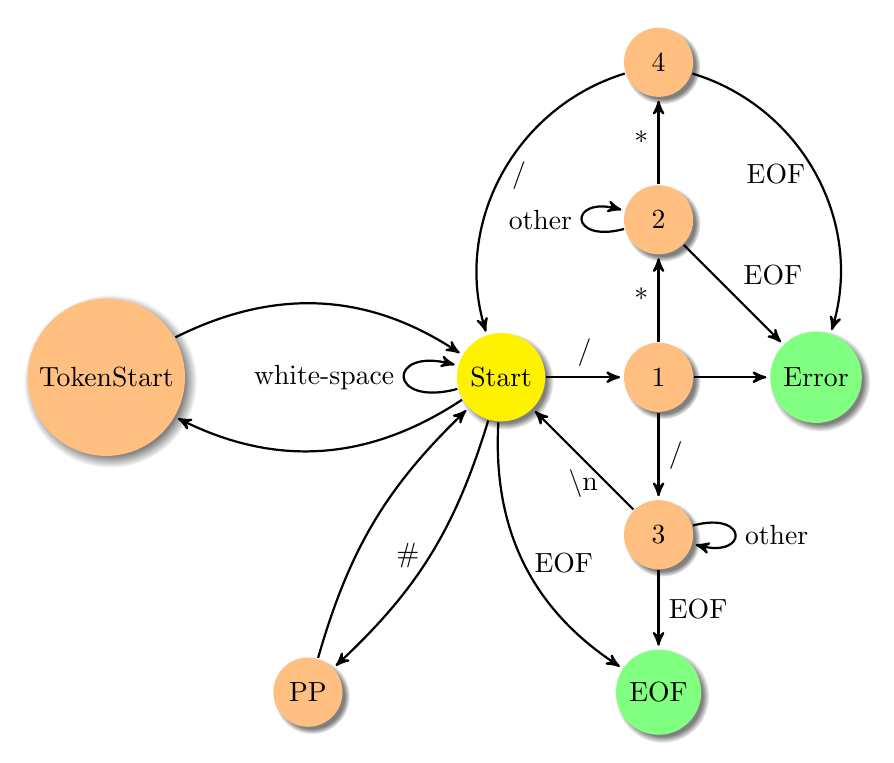
\begin{tikzpicture}[shorten >=1pt,node distance=2cm,on grid,>=stealth',
thick,bend angle=45,
every state/.style={fill,draw=none,orange!50!white,circular drop
    shadow,text=black},
accepting/.style ={green!50!white,text=black},
    initial/.style={yellow,text=black}]
\node[state,initial] (S) {Start};
\node[state] (A) [right=of S] {1};
\node[state] (C) [above=of A] {2};
\node[state] (CPP) [below =of A] {3};
\node[state] (D) [above=of C] {4};
\node[coordinate](P2)[below=of S]{};
\node[coordinate] (P3) [below=of P2]{};
\node[coordinate] (P4) [left=of P3]{};
\node[state] (PP) [left=of P3]{PP};
\node[state,accepting](Err) [right=of A] {Error};
\node[state,accepting](EOF) [below=of CPP] {EOF};
\node[coordinate](P1) [left=of S]{};
\node[state](TS) [left=of P1] {TokenStart};

\path[->] (S) edge node [above] {/} (A)
              edge [bend right=30] node [right] {EOF} (EOF)
              edge [loop left] node {white-space} ()
              edge [bend left=15] node [left]{\#} (PP)
              edge [bend left=30] (TS)
          (PP) edge [bend left=15] (S)
          (TS) edge [bend left=30] (S)
          (A) edge node [left] {*} (C)
              edge node [right] {/} (CPP)
              edge node {} (Err)
          (C) edge node [left] {*} (D)
              edge node [above right] {EOF} (Err)
              edge [loop left] node {other} ()
          (CPP) edge node [below] {$\backslash$n} (S)
                edge node [right] {EOF} (EOF)
              edge [loop right] node {other} ()
          (D) edge [bend right] node [right] {/} (S)
              edge [bend left] node [left] {EOF} (Err);
\end{tikzpicture}
\newpage
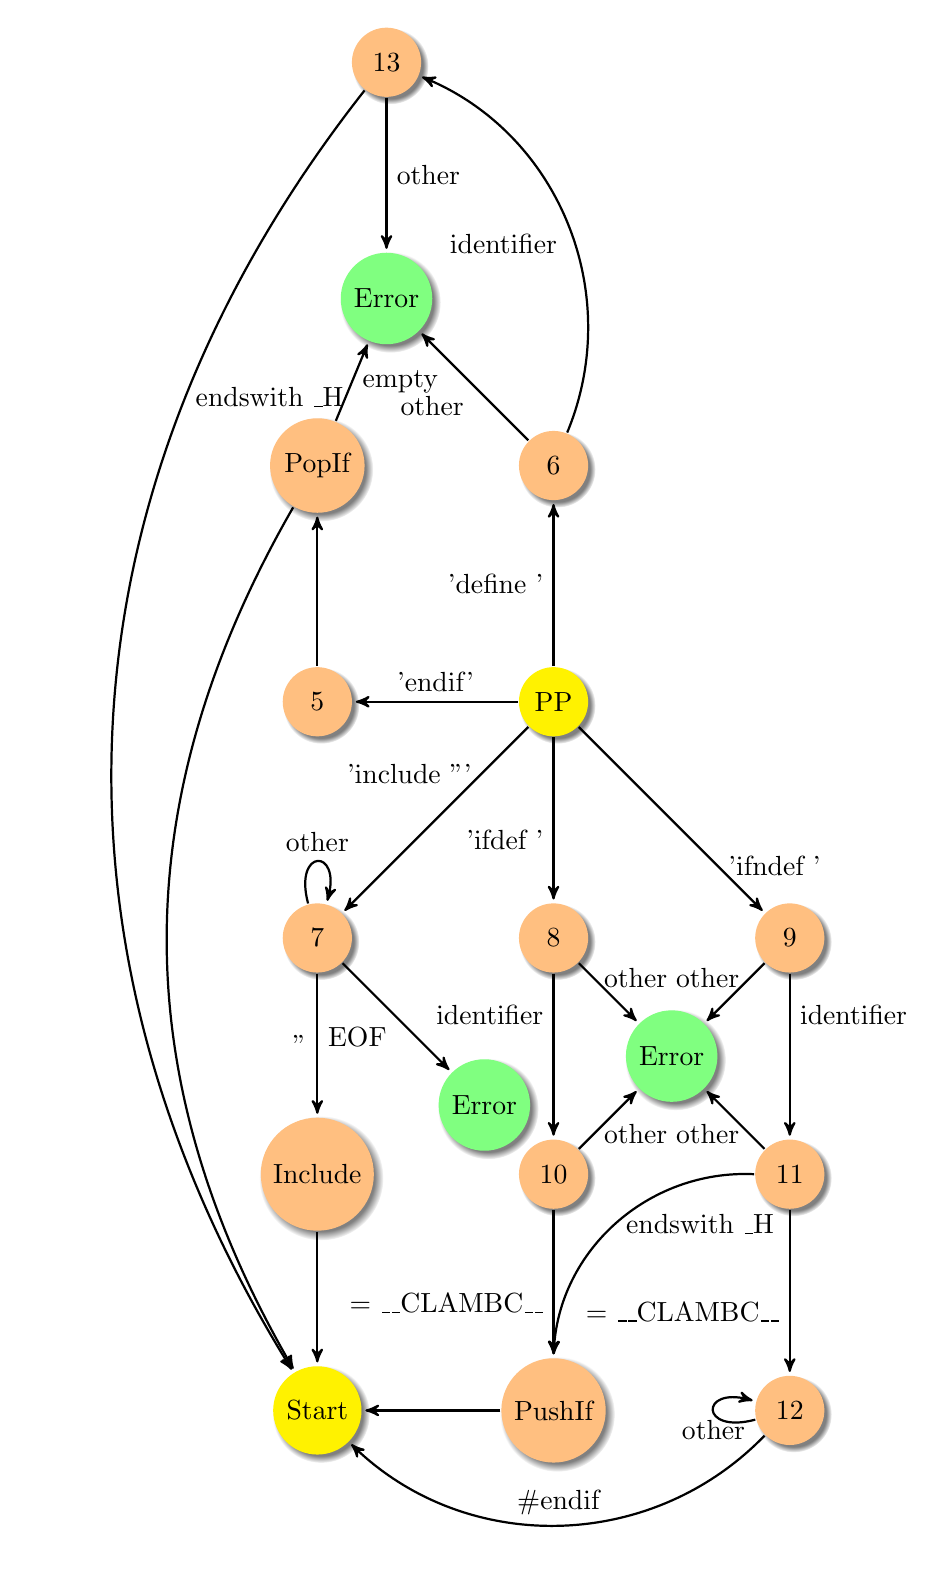
\begin{tikzpicture}[shorten >=1pt,node distance=3cm,on grid,>=stealth',
thick,bend angle=45,
every state/.style={fill,draw=none,orange!50!white,circular drop
    shadow,text=black},
accepting/.style ={green!50!white,text=black},
    initial/.style={yellow,text=black}]


\node[state,initial](PP) {PP};
\node[state](ifdef) [below=of PP] {8};
\node[state](ifndef) [right=of ifdef] {9};
\node[state](endif) [left=of PP] {5};
\node[state](define) [above=of PP] {6};
\node[state](include) [below=of endif] {7};
\node[state](incl) [below=of include] {Include};
\node[state](popif) [above=of endif] {PopIf};
\node[state](id) [below=of ifdef] {10};
\node[state](id2) [below=of ifndef] {11};
\node[state](wait) [below=of id2] {12};
\node[state,accepting](Err3) [above right=1.5cm and 1.5cm of id] {Error};
\node[state](pushif) [below=of id] {PushIf};
\node[coordinate](P20) [left=of define] {};
\node[state,accepting](Err4) [above left=of define] {Error};
\node[state,accepting](Err2) [below right=of include] {Error};
\node[state](id3) [above=of Err4]{13};
\node[state,initial](S) [left=of pushif] {Start};

\path[->]
          (PP) edge node [below left] {'ifdef '} (ifdef)
	       edge node [near end] [right] {'ifndef '} (ifndef)
               edge node [left] {'define '} (define)
	       edge node [near start] [left] {'include "'} (include)
	       edge node [above] {'endif'} (endif)
	  (include) edge node [left] {"} (incl)
	            edge node [below left] {EOF} (Err2)
	            edge [loop above] node {other} ()
	  (incl) edge  node {} (S)
          (endif) edge node {} (popif)
          (popif) edge [bend right=30] node {} (S)
                  edge node [right] {empty} (Err4)
          (ifdef) edge node [near start] [left] {identifier} (id)
                  edge node [near start] [right] {other} (Err3)
          (id) edge node [below left] {= \_\_CLAMBC\_\_} (pushif)
              edge node [near start][right] {other} (Err3)
         (ifndef) edge  node [near start] [right] {identifier} (id2)
                   edge node [near start] [left] {other} (Err3)
          (id2) edge node [below left] {= \_\_CLAMBC\_\_} (wait)
               edge [bend right] node  [right] {endswith \_H} (pushif)
                edge node [near start] [left] {other} (Err3)
          (wait) edge [bend left] node [above] {\#endif} (S)
                 edge [loop left] node [below] {other} ()
%	  (P7.center) edge [bend left=90] node {} (S)
	  (define) edge [bend right] node [below left] {identifier} (id3)
                   edge node [below left] {other} (Err4)
          (id3) edge [bend right=35] node [near start] [right] {endswith \_H} (S)
                edge node [right] {other} (Err4)
          (pushif) edge (S)
     ;

\end{tikzpicture}
\newpage
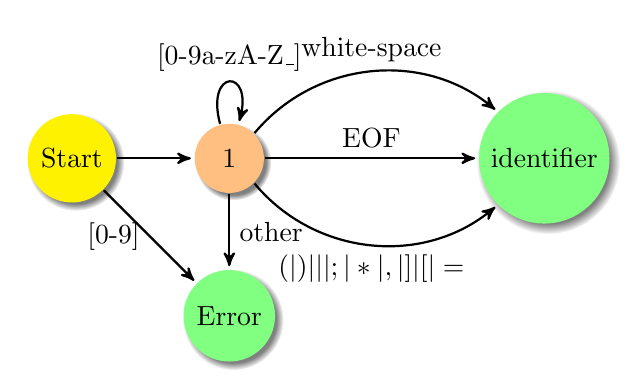
\begin{tikzpicture}[shorten >=1pt,node distance=2cm,on grid,>=stealth',
thick,bend angle=45,
every state/.style={fill,draw=none,orange!50!white,circular drop
    shadow,text=black},
accepting/.style ={green!50!white,text=black},
    initial/.style={yellow,text=black}
    ]
\node[state,initial] (Start) {Start};
\node[state](id) [right= of Start] {1};
\node[coordinate](P1) [right=of id]{};
\node[state,accepting] (identifier) [right of=P1] {identifier};
\node[state,accepting](Err) [below of=id] {Error};

\path[->]
     (Start) edge node [left] {[0-9]} (Err)
             edge (id)
     (id) edge [loop above] node [above]{[0-9a-zA-Z\_]} ()
          edge [bend left] node [above] {white-space} (identifier)
          edge [bend right] node [below] {$(|)|{|}|;|*|,|]|[|=$} (identifier)
	  edge node [above] {EOF} (identifier)
          edge node [right] {other} (Err);
\end{tikzpicture}
\newpage
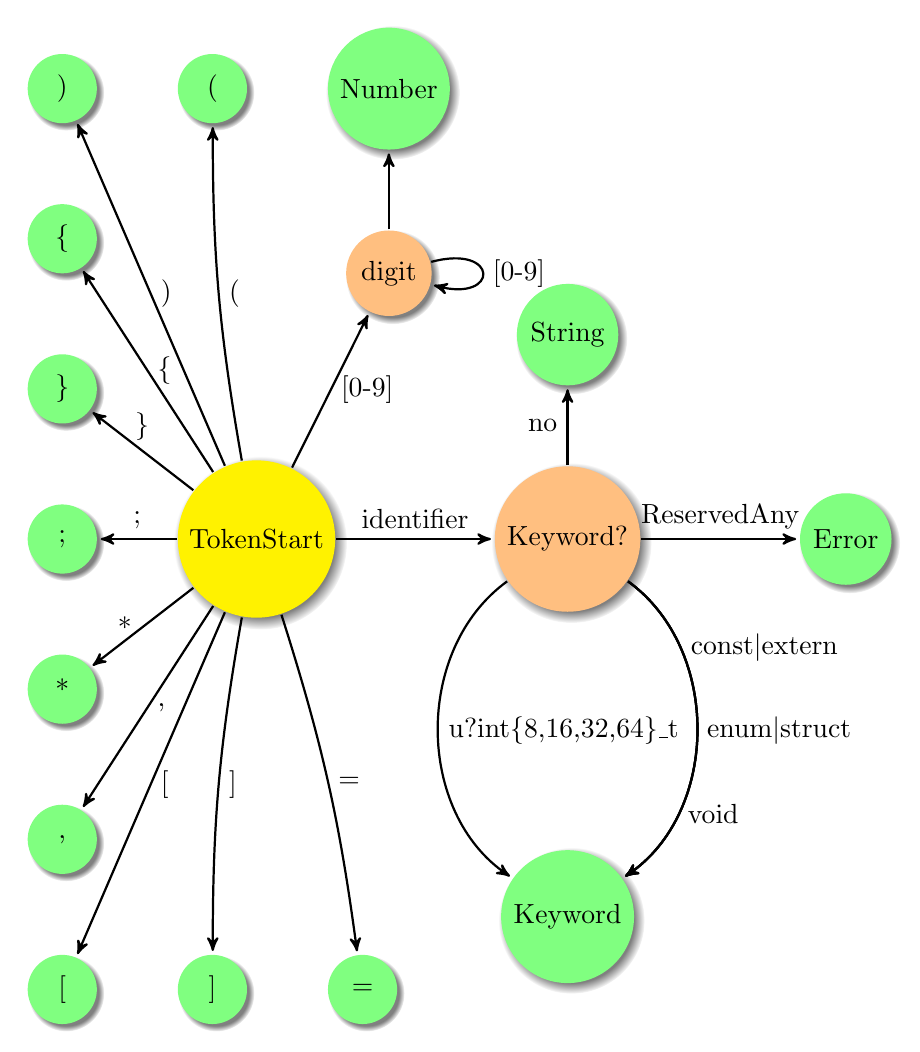
\begin{tikzpicture}[shorten >=1pt,node distance=1cm,>=stealth',
thick,bend angle=45,
every state/.style={fill,draw=none,orange!50!white,circular drop
    shadow,text=black},
accepting/.style ={green!50!white,text=black},
    initial/.style={yellow,text=black}
    ]
\node[state,initial] (TokenStart) {TokenStart};
%\node[state,initial] (Start) {Start};
\node[state](KWQ) [right=2cm of TokenStart] {Keyword?};
\node[state,accepting](Error) [right=2cm of KWQ] {Error};
\node[state,accepting](String) [above= of KWQ] {String};
\node[state,accepting](d5) [left=of TokenStart] {;};
\node[state,accepting](d4) [above=of d5]{\}};
\node[state,accepting](d3) [above=of d4]{\{};
\node[state,accepting](d2) [above=of d3] {)};
\node[state,accepting](d1) [right=of d2]{(};
\node[state,accepting](d6) [below=of d5] {*};
\node[state,accepting](d7) [below=of d6]{,};
\node[state,accepting](d8) [below=of d7]{[};
\node[state,accepting](d9) [right=of d8]{]};
\node[state,accepting](d10) [right=of d9] {=};
\node[state,accepting](number) [right=of d1] {Number};
\node[state](digit) [below=of number] {digit};
\node[coordinate](P1) [below=of KWQ]{};
\node[coordinate](P2) [below=of P1]{};
\node[state,accepting](KW) [below=of P2] {Keyword};

\path[->]
     (TokenStart) edge node [above] {identifier} (KWQ)
     (KWQ) edge node [left] {no} (String)
     (KWQ) edge node [above] {ReservedAny} (Error)
     (TokenStart) edge [bend left=5] node [right] {(} (d1)
		  edge node [right] {)} (d2)
                  edge node [right] {\{} (d3)
                  edge node [above] {\}} (d4)
                  edge node [above] {;} (d5)
                  edge node [left] {*} (d6)
                  edge node [right] {,} (d7)
                  edge node [right] {[} (d8)
                  edge [bend right=5] node [right] {]} (d9)
                  edge [bend left=5] node [right] {=} (d10)
                  edge node [right] {[0-9]} (digit)
     (digit) edge [loop right] node [right] {[0-9]} ()
             edge (number)
    (KWQ) edge [bend right=55] node [right] {u?int\{8,16,32,64\}\_t} (KW)
          edge [bend left=55] node [near start] [right] {const$|$extern} (KW)
          edge [bend left=55] node [right] {enum$|$struct} (KW)
          edge [bend left=55] node [near end] [right] {void} (KW)
    ;
\end{tikzpicture}

\begin{tabular}{ll}
ReservedAny & $::=$ ReservedType\\
	&$\mid$ Reserved\\
	&$\mid$ ReservedCXX\\
ReservedType & $::=$ bool\\
&$\mid$ \_Bool\\
&$\mid$ \_Complex\\
&$\mid$ double\\
&$\mid$ float\\
&$\mid$ int\\
&$\mid$ \_Imaginary\\
&$\mid$ long\\
&$\mid$ short\\
&$\mid$ signed\\
&$\mid$ unsigned\\
Keyword & $::=$ const\\
&$\mid$ enum\\
&$\mid$ extern\\
&$\mid$ int8\_t\\
&$\mid$ int16\_t\\
&$\mid$ int32\_t\\
&$\mid$ int64\_t\\
&$\mid$ struct\\
&$\mid$ uint8\_t\\
&$\mid$ uint16\_t\\
&$\mid$ uint32\_t\\
&$\mid$ uint64\_t\\
&$\mid$ void\\
Reserved & $::=$ $\mid$ auto\\
&$\mid$ break\\
&$\mid$ case\\
&$\mid$ char\\
&$\mid$ const\\
&$\mid$ continue\\
&$\mid$ default\\
&$\mid$ do\\
&$\mid$ double\\
&$\mid$ else\\
&$\mid$ enum\\
&$\mid$ extern\\
&$\mid$ float\\
&$\mid$ for\\
&$\mid$ goto\\
&$\mid$ if\\
&$\mid$ inline\\
&$\mid$ int\\
&$\mid$ long\\
&$\mid$ register\\
&$\mid$ restrict\\
&$\mid$ return\\
&$\mid$ short\\
&$\mid$ signed\\
&$\mid$ sizeof\\
&$\mid$ static\\
&$\mid$ struct\\
&$\mid$ switch\\
&$\mid$ typedef\\
&$\mid$ union\\
&$\mid$ unsigned\\
&$\mid$ void\\
&$\mid$ volatile\\
&$\mid$ while\\
&$\mid$ \_Bool\\
&$\mid$ \_Complex\\
&$\mid$ \_Imaginary\\
&$\mid$ \_\_func\_\_\\
&$\mid$ asm\\
&$\mid$ \_Decimal32\\
&$\mid$ \_Decimal64\\
&$\mid$ \_Decimal128\\
&$\mid$ \_\_alignof\\
&$\mid$ \_\_attribute\\
&$\mid$ \_\_builtin\_choose\_expr\\
&$\mid$ \_\_builtin\_offsetof\\
&$\mid$ \_\_builtin\_types\_compatible\_p\\
&$\mid$ \_\_builtin\_va\_arg\\
&$\mid$ \_\_extension\_\_\\
&$\mid$ \_\_imag\\
&$\mid$ \_\_label\_\_\\
&$\mid$ \_\_real\\
&$\mid$ \_\_thread\\
&$\mid$ \_\_FUNCTION\_\_\\
&$\mid$ \_\_PRETTY\_FUNCTION\_\_\\
&$\mid$ typeof\\
&$\mid$ \_\_private\_extern\_\_\\
&$\mid$ \_\_declspec\\
&$\mid$ \_\_cdecl\\
&$\mid$ \_\_stdcall\\
&$\mid$ \_\_fastcall\\
&$\mid$ \_\_ptr64\\
&$\mid$ \_\_w64\\
&$\mid$ \_\_forceinline\\
ReservedCXX & $::=$ $\mid$ catch\\
&$\mid$ class\\
&$\mid$ const\_cast\\
&$\mid$ delete\\
&$\mid$ dynamic\_cast\\
&$\mid$ explicit\\
&$\mid$ export\\
&$\mid$ false\\
&$\mid$ friend\\
&$\mid$ mutable\\
&$\mid$ namespace\\
&$\mid$ new\\
&$\mid$ operator\\
&$\mid$ private\\
&$\mid$ protected\\
&$\mid$ public\\
&$\mid$ reinterpret\_cast\\
&$\mid$ static\_cast\\
&$\mid$ template\\
&$\mid$ this\\
&$\mid$ throw\\
&$\mid$ true\\
&$\mid$ try\\
&$\mid$ typename\\
&$\mid$ typeid\\
&$\mid$ using\\
&$\mid$ virtual\\
&$\mid$ wchar\_t\\
&$\mid$ alignof\\
&$\mid$ axiom\\
&$\mid$ char16\_t\\
&$\mid$ char32\_t\\
&$\mid$ concept\\
&$\mid$ concept\_map\\
&$\mid$ constexpr\\
&$\mid$ decltype\\
&$\mid$ late\_check\\
&$\mid$ nullptr\\
&$\mid$ requires\\
&$\mid$ static\_assert\\
&$\mid$ thread\_local\\
&$\mid$ \_\_null\\
&$\mid$ \_\_has\_nothrow\_assign\\
&$\mid$ \_\_has\_nothrow\_copy\\
&$\mid$ \_\_has\_nothrow\_constructor\\
&$\mid$ \_\_has\_trivial\_assign\\
&$\mid$ \_\_has\_trivial\_copy\\
&$\mid$ \_\_has\_trivial\_constructor\\
&$\mid$ \_\_has\_trivial\_destructor\\
&$\mid$ \_\_has\_virtual\_destructor\\
&$\mid$ \_\_is\_abstract\\
&$\mid$ \_\_is\_base\_of\\
&$\mid$ \_\_is\_class\\
&$\mid$ \_\_is\_empty\\
&$\mid$ \_\_is\_enum\\
&$\mid$ \_\_is\_pod\\
&$\mid$ \_\_is\_polymorphic\\
&$\mid$ \_\_is\_union

\end{tabular}
\end{document}

\end{document}
